\documentclass[a4paper,english,12pt]{article}
\usepackage{graphicx}
\usepackage[T1]{fontenc}
\usepackage[utf8]{inputenc}
\usepackage{babel}
\usepackage[colorlinks=true]{hyperref}
\usepackage{upgreek} %proper greek letters
\usepackage{fullpage}
\usepackage{lineno}
\usepackage{amsmath} % typesetting math
\usepackage{amssymb}
\usepackage{textcomp}
\usepackage{booktabs} % nice tables
\usepackage[round,sort&compress]{natbib}
\usepackage{pdfpages} %include external pdfs
\usepackage{enumitem} %for noitemsep in lists
\usepackage{csquotes} %for noitemsep in lists
\usepackage{subfig}
\renewcommand{\arraystretch}{1.2} % space in tables
\usepackage{authblk}
\usepackage{multirow}
\usepackage{soul}
\usepackage{amssymb}

\newcommand{\mr}[2]{\multirow{#1}{*}{#2}}  
\newcommand{\mc}[3]{\multicolumn{#1}{#2}{#3}}

% Comments
\newcommand{\ds}[2][orange]{\textcolor{#1}{#2}}
\newcommand{\bh}[2][red]{\textcolor{#1}{#2}}

% \usepackage[toc,page]{appendix} %for appendix titles
% \usepackage[titletoc,title]{appendix} %for appendix titles
\usepackage[colorinlistoftodos,prependcaption,textsize=tiny]{todonotes} %todo note in margin
\newcommand{\answ}[1]{\todo[linecolor=blue,backgroundcolor=blue!25,bordercolor=blue]{#1}}

\begin{document}

\title{Analytical and Monte-Carlo modeling of Multi-Parallel Slit and Knife-Edge Slit Prompt Gamma Cameras}

\author[1,2]{Brent F. B. Huisman}
\author[2]{\'E. Testa}
\author[3]{D. Dauvergne}
\author[1]{J.~M. L\'etang}
\author[1]{D. Sarrut}
\affil[1]{~CREATIS, Universit\'e de Lyon; CNRS UMR5220; INSERM U1206; INSA-Lyon; Universit\'e Lyon 1; Centre L\'eon B\'erard, Lyon, France}
\affil[2]{~IPNL, Universit\'e de Lyon; CNRS/IN2P3 UMR5822; Universit\'e Lyon 1 Lyon, France}
\affil[3]{~ Laboratoire de Physique Subatomique et de Cosmologie, CNRS/IN2P3, Grenoble, France}
\affil[ ]{~E-mail: e.testa@ipnl.in2p3.fr}

\maketitle

\begin{abstract}

\emph{Purpose:} 

\emph{Materials and Methods:} 

\emph{Results:} 

\emph{Conclusion:} 

\end{abstract}

\tableofcontents

\newpage

%%%%%%%%%%%%%%%%%%%%%%%%%%%%%%%%%%%%%%%%%%%%%%%%%%%%%%%%%%%%%%%%%%%%%%%%%%%%%%%%
\section{Introduction}

The well-defined range of particles in matter is the main reason they are used in cancer treatment today. Unfortunately we are not able to take full advantage of this property, because of treatment uncertainties, e.g. uncertainties in patient positioning, changes of patient anatomy between treatment fractions and uncertainties in the Hounsfield unit to particle stopping power conversion \citep{Paganetti2012}. Often, medical practice leads to the use of several irradiation fields to ensure robust treatment planning at the expense of larger doses in healthy tissue in respect to ideal treatment with single irradiation field. Moreover margins around the tumor are added, reducing the potential benefits of particle treatment \citep{Knopf2013}. Ion-range verification could permit more precise planning which could take maximum advantage of the steep Bragg peak (BP) fall-off and reduce damage to tissues surrounding the tumor. A promising modality to perform this verification consists in detecting prompt gammas (PGs), a natural byproduct in particle treatments \citep{Krimmer2017a, Parodi2018}. Various modalities are currently under investigation and can be classified in two categories: imaging devices using either mechanical or electronical collimation (respectively collimated \citep{Perali2014, Min2012, Pinto2014a} and Compton cameras \citep{Krimmer2015,Kurosawa2012,Thirolf2016,Polf2015,Llosa2016}) and non-imaging devices such as Prompt Gamma Spectroscopy (PGS) \citep{Hueso-Gonzalez2016}, Prompt Gamma Timing (PGT) \citep{Pausch2016} and Prompt Gamma Peak Integral (PGPI) \citep{Krimmer2017}. Regarding cameras using mechanical collimators, two types of designs have been considered: Multi-Parallel Slit (MPS) and Knife-Edge Slit (KES). The latter has been chosen by the IBA group to be prototyped and has been tested during treatment of patients \ds{(only one patient ?)}\bh{fixed wording.} at OncoRay in Dresden, Germany. Both types of collimators provide part or the whole of the one-dimensional PG profile along the beam direction.

To date, three publications \citep{Smeets2016, Lin2017, Park2017} have attempted to compare these two types of collimators with various geometries. Indeed, although they refer to the same KES design from \citep{Perali2014} some geometrical parameters are slighlty different in \citep{Lin2017, Park2017} (i.e. the source-collimator distance and the collimator-absorber distance). The same applies for the MPS design: \cite{Smeets2016} uses a modified MPS design from \cite{Pinto2014a}, \cite{Lin2017} used the design from \cite{Gueth2013} and \cite{Park2017} their own specific design. It is worth to note that the authors of the latter publication justified the need for a complementary study by the fact that the MPS geometries used in \cite{Smeets2016, Lin2017} were not \enquote{optimized}. 
Unfortunately the fact that the optimizations of KES and MPS designs were not performed according the same figures of merit can not ensure a fair comparison of the two designs. Actually from a general point of view the design of any collimated device is a compromise between detection efficiency and spatial resolution. While collimator features have been extensively investigated in the context of nuclear imaging \citep{Gunter2004}, no theoretical considerations have been proposed for the specific 1D collimation systems developed in the context of ion-range verification during hadrontherapy.

Therefore, the first objective of this article is to present an analytical model based on geometrical considerations that allows for a theoretical estimation of the detection efficiency and spatial resolution, for both MPS and KES designs. The intrinsic features of MPS and KES collimators are then derived and the model is validated by means of Monte Carlo (MC) simulations. In light of the predictions of this analytical model, the PG prototypes developed by the CLaRyS collaboration and the IBA group are compared and their performances are assessed in terms of detection efficiency, spatial resolution and fall-off retrieval precision thanks to MC simulations.

%     \item Validate the analytical model using MC studies.

% \begin{itemize}
%   \item Develop an analytical model based on geometric considerations
%   \begin{itemize}
%   	\item The model should allow for a theoretical estimation of the detection efficiency and spatial resolution, for both MPS and KES and so allow for conclusions to be drawn about the intrinsic features of MPS and KES collimators.
%     \item Validate the analytical model using MC studies.
%     \item Address deficiencies in previous studies. In \cite{Smeets2016} and \cite{Lin2017}: the KES/MPS detection efficiency ratio is 1.6 for Smeets 2016 and 5.3 for Lin 2017, assuming the use of the same energy window\todo{was it the same energy window?}\answ{I think so. Certainly for Smeets 2016}. These comparisons were not performed under identical conditions, nor were differences accounted for.
%   \end{itemize}
%   \item Prototype comparison
%     \begin{itemize}
%     	\item The clinically relevant parameter is, currently, the fall-off position (FOP), allowing for a BP verification. The prototypes will thus be compared on that merit.
%     \end{itemize} 
%   
% \end{itemize}  


%Taking a step back, the 1D PG signal can be paramatrized, as well as the relevant dimensions of the PG collimator. A simple model could be built relating these factors which in turn can be tested in a study. This publication will demonstrate and validate a model for a knife-edge slit (KES) and multiparallel slit (MPS) collimator designs, both analytically and by using Monte Carlo (MC) studies. The objectives of the present paper are the following:



%%%%%%%%%%%%%%%%%%%%%%%%%%%%%%%%%%%%%%%%%%%%%%%%%%%%%%%%%%%%%%%%%%%%%%%%%%%%%%%%
%%%%%%%%%%%%%%%%%%%%%%%%%%%%%%%%%%%%%%%%%%%%%%%%%%%%%%%%%%%%%%%%%%%%%%%%%%%%%%%%
%%%%%%%%%%%%%%%%%%%%%%%%%%%%%%%%%%%%%%%%%%%%%%%%%%%%%%%%%%%%%%%%%%%%%%%%%%%%%%%%

\section{Materials and Methods}

\subsection{Analytical model for spatial resolution and detection efficiency}

%Camera performance is mainly characterized by a compromise between spatial resolution and detection efficiency. During camera design, modifications of some geometrical parameters, such as collimator-crystal distance, collimator pitch or depth\dots, often lead to improvement of one of this criteria and deterioration of the other. 

In order to compare performance of different camera types and configurations, we derive an analytical model that predict camera performances. Such models allow to estimate variation in performance according to variation in geometrical parameters assuming perfect gamma detection in the absorber (full gamma absorption on the absorber entrance surface). Figure~\ref{fig:CamerasParameters} presents the schemes of the MPS and KES cameras gathering the geometrical parameters defined in Table~\ref{table:CamerasParameters}.

\begin{figure}[htbp]
    \centering
    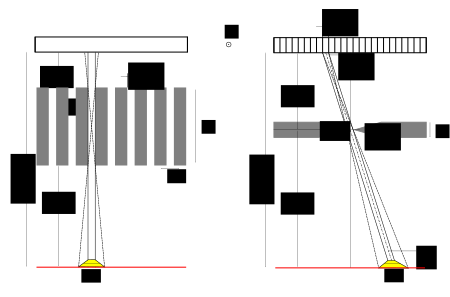
\includegraphics[width=.8\textwidth]{MPS-KES_scheme}
    \caption{Schemes of the Multi-Parallel Slit (MPS) and the Knife-Edge Slit (KES) cameras. The definition of the various parameters is given in Table~\ref{table:CamerasParameters}. The red line corresponds to a linear source perpendicular to the slit camera planes. $\Lambda$ is the the distance between the source point and the middle of the absorber entrance surface in the KES.}
    \label{fig:CamerasParameters}
\end{figure}    

\begin{table}[h]
\centering
\begin{tabular}{lllll}
	\midrule
																& MPS               & KES \\
	\midrule
	Source-collimator distance		& $d_1$             & $d_1'$ \\
 	Collimator-absorber distance	& $d_2$             & $d_2'$ \\
	Source-absorber distance			& $L=d_1+D+d_2$			& $L=d_1'+d_2'$\\
 	Collimator thickness 					& $D$               & $T$ \\
	Camera pitch									& $p$								& $p'$\\
	Knife-edge slit angle					& $\varnothing$			& $\alpha$\\	
	%\cline{2-3}
	Slit width										& s & s \\ %\multicolumn{2}{c}{s} \\
	\midrule
\end{tabular}
\caption{Geometrical parameters of the MPS and KES cameras. One can also define the fill factor $f$ of the MPS collimator: $f=(p-s)/p$ (ratio between the septa width and the pitch). It is worth to note that the source-collimator distance and the collimator-absorber distance are not defined exactly in the same way in the two collimator designs.}
\label{table:CamerasParameters}
\end{table}



\subsubsection{Spatial resolution}

\newcommand\FOV{\textrm{Res}}
\newcommand\MPS{\textrm{MPS}}
\newcommand\KES{\textrm{KES}}
%\newcommand\du{\textrm{du}}
\newcommand\du{}
\newcommand\DE{\textrm{Eff}}

From a geometrical point of view, the spatial resolution, denoted $\FOV_{\du}$, is characterized by the \textit{detector unit field of view}. This is the portion of
the source that can be seen through a single camera unit: a single slit for the MPS and a single detector unit for the KES. The probability of a photon emitted at a
given point along a linear source perpendicular to the slit plane to reach
this detector unit can be described as an isosceles trapezoid whose width of the top segment corresponds to the slit width while the width of the base segment is equal to the sum of the slit width and the penumbra. We defined $\FOV_{\du}$
as the FWHM of this trapezoid, see eq~\ref{eq:fov_mps} and \ref{eq:fov_kes}.

\begin{eqnarray}
  \label{eq:fov_mps}
  \FOV_{\du}^{\MPS} & = & s\left(1+ \frac{d_1}{D}\right) = p(1-f) \frac{D+d_1}{D} \\
  \label{eq:fov_kes}
   \FOV_{\du}^{\KES} & = & s\left(1+ \frac{d_1'}{d_2'}\right) = \frac{sL}{d_2'}
\end{eqnarray}

If collimator transparency is neglected, $\FOV_{\du}$ is fully defined by geometrical parameters, in particular the slit width $s$. However, prompt gamma have high penetration capability that can not be neglected in the case of KES where the collimator depth is very small in the region of the knife edge around the slit. Indeed, we define the \textit{Effective Slit Opening} $s_e$ that can be used in the evaluation of the field of view and the efficiency in place of the geometrical slit width. \cite{Metzler2005}
proposed a method to estimate the effective slit width, specifically to calculate
the spatial resolution accurately. The proposed expressions were based on
one-dimensional cuts through the pinhole geometry and can be applied directly to
a knife-edge geometry without modification. Their approach is for a point source
and dependent on the location of the source within the \FOV. For a source in the
center, it simplifies to eq.~\ref{eq:se} with $\mu$ the linear attenuation
length of the collimator material.

\begin{eqnarray}
  s_e & = & s + \frac{\ln2}{\mu\tan\alpha}   \label{eq:se} \\
   \FOV_{\du}^{\KES} & = & s_e\left(1+ \frac{d_1'}{d_2'}\right) = \frac{s_eL}{d_2'}          
  \label{eq:fov_kes_se}
\end{eqnarray}

Hence, eq.~\ref{eq:fov_mps} and eq.~\ref{eq:fov_kes_se} represent the spatial resolution of the MPS and KES camera systems according to simple geometrical and gamma attenuation parameters (collimator distances, angle and collimator linear attenuation length). The spatial resolution is expressed in millimeters. 

\subsubsection{Detection efficiency}

The probability that a gamma reaches a given detector unit is described by the solid angle $\Omega_D$ of the detector unit in respect to the gamma emission point.

For MPS, the solid angle is composed of the azimuthal angle and the polar angle. With small angle approximation, it is described by
eq.~\ref{eq:solid_angle_mps}. Note that this is true only when $\Omega_D$ is
limited by the slit width, i.e. the absorber size and the distances (e.g. $L$ and $D$) are such that
all photons that cross the collimator impinge on detector material. 

For KES, the solid angle under which a point of the source sees a detector unit depends on the location of the point source, $x$, since the distance between source and detector changes significantly over the field of view of the camera. We
consider the solid angle for a point of the source that is within the central
part of the field of view of the crystal at location $x$ on the detector plane
(the origin of the detector plane facing the center of the slit). Under small
angle approximation, the solid angle is given by eq.~\ref{eq:solid_angle_kes}. \ds{it is a kind of upper bound on the DetEff, right ? }

\begin{align}  
  \Omega_D^{\MPS} & = \frac{H}{L} \frac{s}{D+d_1} \label{eq:solid_angle_mps} \\
	\Omega_D^{\KES} & = \frac{H L p'}{\Lambda^3(x)} =  \frac{H p'}{L^2 \left( 1+\frac{x^2}{d_2^{'2}} \right)^{3/2}} \label{eq:solid_angle_kes} 
\end{align}
with $\Lambda$ the distance between the source point and the crystal in the KES.


Since we are interested in extended gamma emission source, let us consider now a linear source in front the cameras (red lines in Figure~\ref{fig:CamerasParameters}). In this case, the camera detection efficiency is determined not only by the point source detection efficiency (PSDE) characterized by $\Omega_D$, but also by the fraction of the source seen by the camera (the FOV factor) $f_{\textrm{FOV}} = \frac{\FOV_{\du}}{p}$ where $p$ is the pitch of the camera. It is, in principle, larger than 1 since cameras are usually designed to see all the source without any hidden regions.

Hence, the detection efficiency of a detector unit ($\DE_{\du}$) and therefore the detection efficiency of the whole camera located in front a linear source perpendicular to  the camera plane can be expressed as:
\begin{align} 
	\DE_{\du} = \textrm{PSDE} \times f_{\textrm{FOV}}
\end{align}
with $\textrm{PSDE}$ the detection efficiency for a point-like source that sees a detector through the slit, and $f_{\textrm{FOV}} = \frac{\FOV_{\du}}{p}$ the FOV factor. The detection efficiency of MPS and KES are given by eq.~\ref{eq:de_mps} and~\ref{eq:de_kes}, respectively.

\begin{eqnarray}
  \label{eq:de_mps}
  \DE_{\du}^{\MPS} & = & \frac{\Omega_D^{\MPS}}{4\pi} \frac{\FOV_{\du}^{\MPS}}{p} \nonumber\\
                & = & \frac{1}{4\pi} \frac{H}{L} \frac{s}{D+d_1} p(1-f)
                      \frac{D+d_1}{D} \frac{1}{p} \nonumber\\
                & = & \frac{Hs(1-f)^2}{4 \pi L D}
\end{eqnarray}

\begin{eqnarray}
  \label{eq:de_kes}
	\DE_{\du}^{\KES} & = & \frac{\Omega_D^{\KES}}{4\pi} \frac{\FOV_{\du}^{\KES}}{p'} \nonumber\\
	& = & \frac{s_e H}{4\pi d_2' L} \frac{1}{\left( 1+\frac{x^2}{d_2^{'2}}\right)^{3/2}}
\end{eqnarray}


% As a conclusion, spatial resolution of MPS and KES camera are given by
% eq.~\ref{eq:fov_mps} and \ref{eq:fov_kes_se}, and detection efficiency are given
% eq.~\ref{eq:de_mps} and \ref{eq:de_kes}. Other non geometrical parameters, such
% as type of crystal, energy thresholds or TOF thresholds are also important and
% will be discussed later. The next section describes the Monte-Carlo simulations that have been
% performed to evaluate this analytical model and a comparison between MPS and KES
% systems.

The formulas of detection efficiency and spatial resolution of MPS and KES cameras are gathered in Table~\ref{table:AMformulas}. The most striking feature of theses 
formulas is their similarities. 

\begin{table}[h]
\centering
\begin{tabular}{lll}
	\midrule
	                            & MPS                              & KES \\
	\midrule
	Effective slit width ($s_e$)& $s$                              & $s + \frac{\ln(2)}{\mu \tan(\alpha)}$ \\
 	Spatial resolution (Res)		& $s \left(1+\frac{d_1}{D}\right)$ & $s_e \left( 1+\frac{d_1'}{d_2'} \right)$ \\
	Detection efficiency (Eff)	& $\frac{H s}{ 4 \pi L D } (1-f) $ & $\frac{H s_e}{ 4 \pi L d_2' } \left( 1 + \frac{x^2}{d_2^{'2}} \right)^{-3/2} $ \\
 	Collimator effective thickness ($T_e$) & $D\times f$           & $T$ \\
	\midrule
\end{tabular}
\caption{MPS and KES detection efficiencies and spatial resolutions from the analytical model. The parameters of the cameras are defined in figure~\ref{fig:CamerasParameters}. $\mu$ is the linear attenuation length of the collimator material.}
\label{table:AMformulas}
\end{table}

To be more specific, let us define the following conditions that we will refer to as \enquote{MPS and KES Similarities Conditions} (MKSC):
\begin{itemize}
	\item same distance between the source and the MPS collimator entrance and between the source and the middle of the KES collimator: $d_1=d_1'$ ;
	\item MPS collimator thickness equal to the KES collimator-absorber distance: $D=d_2'$ ;
	\item same source-absorber distance $L$ (which entails $d_2=0$ with the previous conditions), same height $H$ and same slit width $s$.	
\end{itemize}
We can also consider perfect collimator condition (PCC) for which the collimators present infinite absorption capacity. In this condition, $s_e=s$ and the filling factor $f$ of the MPS can be decreased down to zero without degrading the collimation properties.

Combining these conditions (MKSC and PCC) then MPS and KES have strictly the same spatial resolution (Res) and the same detection efficiency (Eff) in the central part of the cameras ($x=0$). The main deviations between the actual MPS and KES performances are the following: 
\begin{itemize}
	\item the partial transparency of the collimators leads to:
	\begin{itemize}
		\item an effective slit width of KES larger than the one of the MPS. In the case of the KES prototype of the IBA group, the term accounting for collimator transparency $\left(\frac{\ln(2)}{\mu \tan(\alpha)}\right)$ is about 5~mm (with $\mu\sim 8\times10^{-1}$~cm$^{-1}$ for the tungsten alloy in the 3-6~MeV range and $\alpha=63$\textdegree) meaning that the effective slit $s_e$ is about twice the actual slit width ($s=6$~cm).
		\item an actual fill factor that cannot be neglected: in the case of the MPS prototype of the CLaRyS collaboration it can adjusted but a standard value is 0.4, leading to an actual detection efficiency about half the one of the perfect MPS collimator with $f=0$. 
	\end{itemize}
	\item the KES design intrinsically leads to a detection efficiency that decreases when the source moves away from the center of the camera while the MPS detection efficiency remains constant over the whole camera field of view.
\end{itemize}
It is worth to note that the partial transparency of the collimators leads to an increase of the KES spatial resolution (Res) and a decrease of the MPS detection efficiency (Eff) with similar amplitudes (factor of 2). Since both Res and Eff are proportional to the slit width $s$ one can expect that KES and MPS designs fulfilling MKSC should have very close actual performances if the KES slit width corresponds to the half of the MPS slit width. 

For illustration purposes, Figure~\ref{fig:AMpredictions} \answ{Figure to be improved if we think it is interesting \ds{YES ! very interesting} \bh{figure looks good to me, I see far, far worse in medical physics ;)}} shows the analytical model predictions for the MPS and KES designs compared in \citep{Smeets2016, Lin2017, Park2017}. Parameters have been extracted from the publications \ds{Maybe a table with the values for all parameters ?}\bh{these parameters are the expressions found in table 2}. We can observe the compromise between detection efficiency and spatial resolution: the designs chosen in these comparisons lead to $\DE_{\du}^{\KES}$ and $\FOV_{\du}^{\KES}$ larger than MPS ones by factors ranging from $\sim3$ to $\sim7$. The detection efficency obtained by \cite{Park2017} is much larger than the other ones due to camera height ($H$) increased by a factor of 2. 

\begin{figure}[!htp]
  \centering
  \subfloat[Detection efficiency]{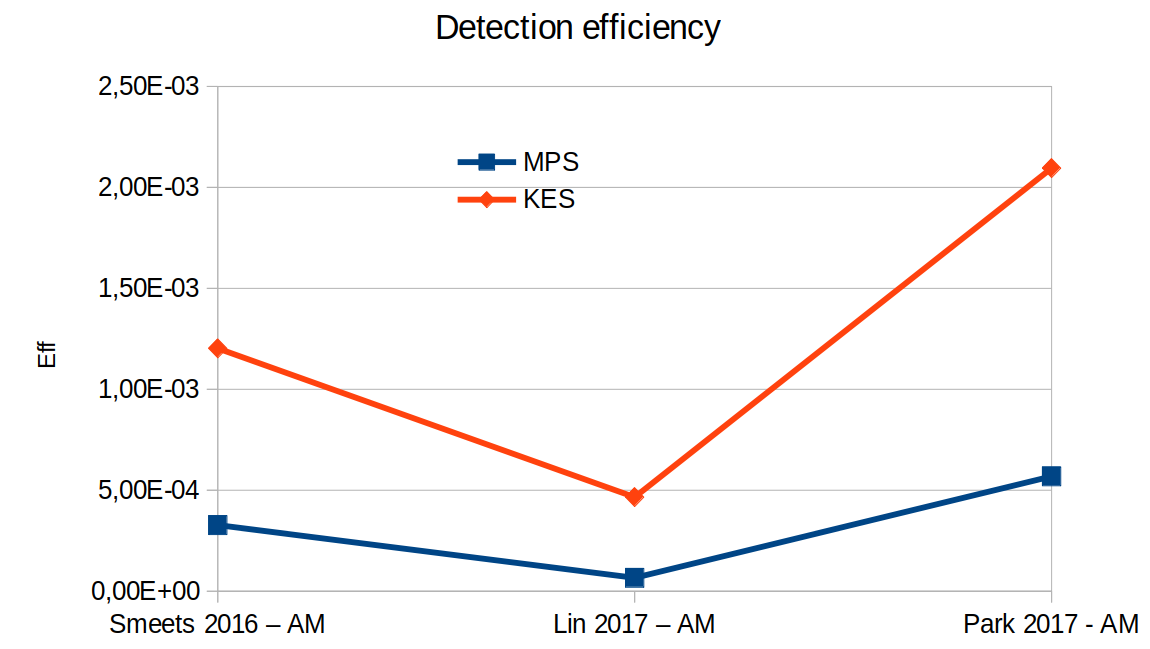
\includegraphics[width=.45\textwidth]{AMpredictionsForConfingurationInLitterature_Eff}}\quad
  \subfloat[Spatial resolution]{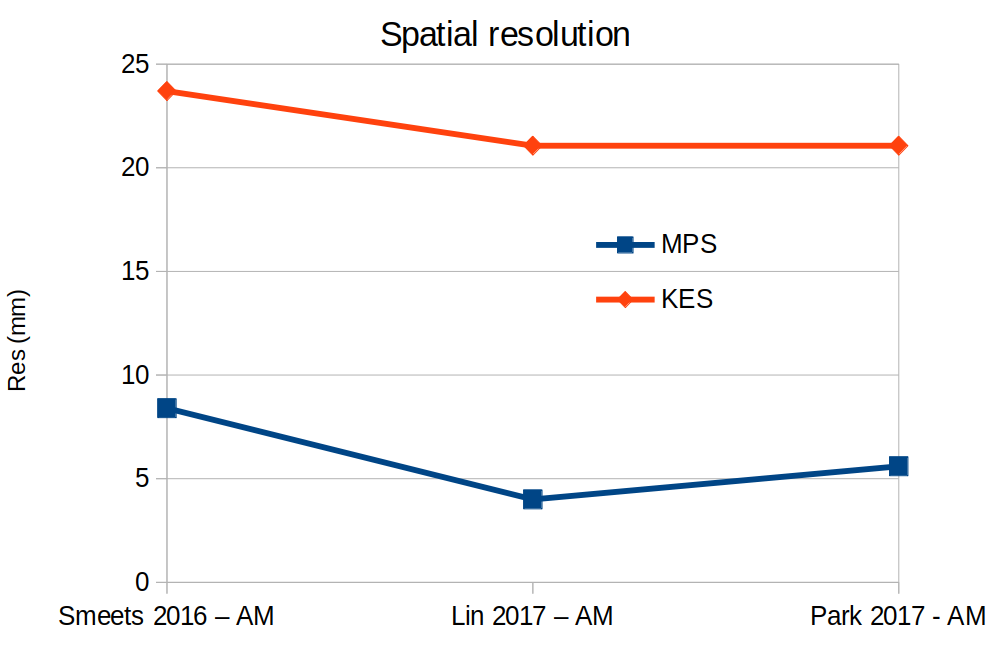
\includegraphics[width=.45\textwidth]{AMpredictionsForConfingurationInLitterature_Res}}
  \caption{\label{fig:AMpredictions} Analytical model predictions for the MPS and KES designs compared in \citep{Smeets2016, Lin2017, Park2017}.}
\end{figure} 

% \begin{table}[h]
% \centering
% \begin{tabular}{|l|l|l|l|l|l|l|l|l|l|l|}
% 	\hline
% 	\mc{2}{|c|}{References}	& \mc{3}{|c|}{\citep{Smeets2016}}										& 	\mc{3}{|c|}{\citep{Lin2017}} 								& 	\mc{3}{|c|}{\citep{Park2017}} \\		
% 	\hline
% 	\mc{2}{|c|}{} 					&	MPS	& KES	& KES/MPS 														& 	MPS	& KES	& KES/MPS 													& 	MPS	& KES	& KES/MPS 						 \\
%  	\hline
% 	Res (mm)	& AM        	& 8.4	& 23.7 & 2.8                  							& 4.0	& 21.1	& 5.3																& 5,6	& 2.1	& 3.8\\
% 	\cline{2-11}
% 						& published		& \mc{3}{|c|}{}																		& \mc{3}{|c|}{}																		& 6.2	& 2.1		& 3,3 \\
% 	\hline
% 	Eff 			& AM        	& $3.7\times10^(-4)$	& $1.2\times10^(-3)$ & 3.26  & $8.9\times10^(-5)$	& $4.7\times10^(-4)$ & 5.2	&$7.7\times10^(-4)$	& $2.6\times10^(-3)$ & 3.4 \\
% 						& published		& \mc{3}{|c|}{}																		& \mc{3}{|c|}{}											& 6.2	& 2.1		& 3,3 \\
% 	\hline
% \end{tabular}
% \caption{MPS and KES detection efficiencies and spatial resolutions from the analytical model. The parameters of the cameras are defined in figure~\ref{fig:CamerasParameters}. $\mu$ is the linear attenuation length of the collimator material.}
% \label{table:AMformulas}
% \end{table}


% Estimate the MPS and KES performances in Smeets 2016 and Lin 2017: the KES/MPS detection efficiency ratio is 1.6 for Smeets 2016 and 5.3 for Lin 2017 (assuming the use of the same energy window) $\Rightarrow$ these comparisons were unfair\dots \answ{TO BE COMPLETED by Etienne}

In the following, we compare the analytical model with MC simulations. We estimate, at first order, the intrinsic efficiency of the MPS and KES absorbers with the Beer-Lambert law assuming that a photon is detected as soon as it reaches the detector. At 4~MeV, the MPS absorber of the CLaRyS collaboration and the KES absorber of the IBA group have intrinsic efficencies of 56\% and 57\% (respectively 3~cm thick BGO scintillators and 3~cm LYSO scintillators).


%%%%%%%%%%%%%%%%%%%%%%%%%%%%%%%%%%%%%%%%%%%%%%%%%%%%%%%%%%%%%%%%%%%%%%%%%%%%%%%%

\subsection{Monte Carlo simulations}
\label{sec:MC}
% 
% \begin{itemize}
%   \item Analytical model verification (AMV): Fair comparison of the two types of collimators with MC simulations. What does it mean? 
%   \begin{itemize}
%     \item Use of same absorbers (the LYSO absorber of the KES prototype that we can consider as the reference), the same energy selection which was not the case in Lin 2017 and the same TOF selection (no TOF)
%     \item Then a discussion of the results in the light of the analytical models
%     \item Note: the KES background level can be obtained from Figure 18 in
%       Perali 2014. Regarding the MPS background level I propose to use the same
%       level as the one of KES for the following reasons: i)
%       the background level in the MPS camera is derived in Pinto 2014 from measurements with large detectors by assuming that the background is proportional to the detector volume. If we apply the same approach, it is reasonable to use the same background levels since we use the same absorbers for MPS and KES. One can argue that the MPS and KES collimators are different. It is true and it is difficult to say whether the larger amount of material in the CLaRyS MPS collimator leads to a larger background with more neutron-induced gammas or a lower background due to a larger attenuation of these gammas\dots At first order the background levels should be similar and a first order estimate is sufficient for a paper that mainly aims at comparing the signal detection of the two cameras.
%   \end{itemize}    
%   \item Simulations of the two prototypes as they are published (results of the submitted paper with the \enquote{regular} cylindrical PMMA target of 15 cm diameter and 20 cm lenght). 
%   \begin{itemize}
%     \item $\Rightarrow$ Comparison of the two prototypes
%     \item Note that the absorbers have different thicknesses
%   \end{itemize}     
% \end{itemize}
The objective of MC simulations is twofold: the analytical model verification (AMV) and the comparison of the MPS and KES prototypes developed by the CLaRyS collaboration and the IBA group, respectively. These two studies use slightly different setups that will be detailed in the following subsections.

\subsubsection{Simulation tool}\label{sec:SimTool}

Imaging paradigms such as PG detection are evaluated against experiments, and often also with Monte Carlo (MC) simulations %~\citep{Moteabbed2011,Gueth2013,Robert2013,Golnik2014a,Janssen2014}. 
For rarely occurring processes such as PG simulation, convergence to the truth to within acceptable statistical error can be slow. Therefore, we used in this study the vpgTLE variance reduction method described in \cite{Huisman2016}. vpgTLE is a two stage process, where firstly a PG yield distribution image is estimated, which in the second stage is used as a PG source. Gate 7.2~\citep{Sarrut2014} with Geant 4.10.02 and the QGSP\_BIC\_HP\_EMY physics list, commonly used for PG studies, are used in this work. Thanks to vpgTLE, simulations for about $10^9$ protons (about $6\times10^8$ photons) took 1-2 hours on a single core of an Intel(R) Core(TM) i7-3740QM.

%%%%%%%%%%%%%%%%%%%%%%%%%%%%%%%%%%%%%%%%%%%%%%%%%%%%%%%%%%%%%%%%%%%%%%%%%%%%%%%%
%\subsubsection{PG camera modeling}\label{sec:camera}

\subsubsection{Prototypes comparison}\label{sec:camera} % paragraph

The MPS and KES prototypes are illustrated in Figure~\ref{fig:detectors}.

\begin{figure}[htp]
  \centering
  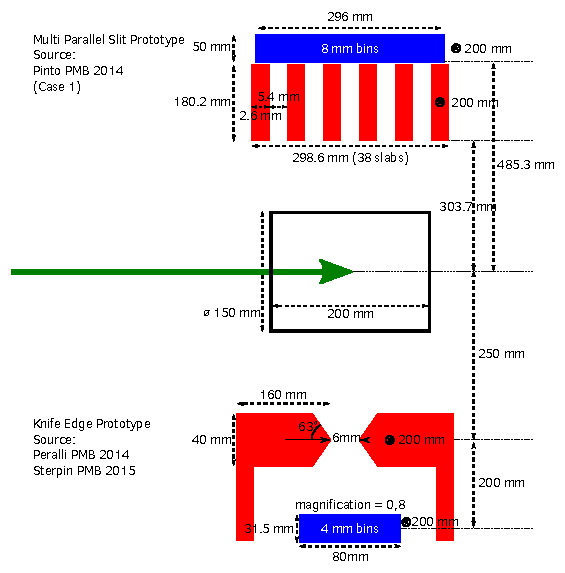
\includegraphics[width=0.8\linewidth]{detectors_cyl}
  \caption{Schematic presentation of the two PG cameras considered in this study. The green arrow represents the proton beam. In red the collimation elements and in blue detection elements. The dimensions were taken from \cite{Pinto2014a} and \cite{Perali2014,Sterpin2015}. Note that the two cameras have an identical detector height ($\odot$ symbol), the two cameras were positioned at an identical location above the head during all simulations, and that here they are not drawn to scale.}
  \label{fig:detectors}
\end{figure}

\paragraph{The MPS prototype developed by the CLaRyS collaboration.}
This camera intends to measure the whole PG profile to control ion-ranges in the patient with a field of view (FoV) of 300 mm. It consists of a bismuth germanium oxide (BGO) absorber and a tungsten alloy collimator. Each block has a sensitive volume of 3.5$\times$3.8$\times$3 cm$^{3}$ and is streaked in 8$\times$8 pseudo-pixels of 4~mm in edge. In the optimization carried out by \cite{Pinto2014a}, parameters such as collimator pitch, axis-to-collimator and axis-to-detector were varied, and their impacts evaluated in terms of fall-off retrieval precision (FRP) and spatial resolution (sharpness of the fall-off region). Here, configuration 1 (with relaxed constraints on spatial resolution) was chosen for its better FRP performance. One can notice that the pitch of the camera (8~mm) corresponds to a whole number of the BGO pseudo-pixel size (4~mm). The event selection from the gamma energy deposition $E$ in the absorber is $E>1$~MeV. Finally this prototype makes use of ToF selection to reduce the neutron background. For the IBA C230 accelerator with a period of 10 ns, \cite{Pinto2014a} chose a window of 4 ns around the PG maximum, based on experimental ToF spectra. This means that about 60\% of the noise could be removed.

%As was done by \cite{Pinto2014a}, the camera lengths (collimator and scintillator volume) are chosen \emph{up to} 300 mm, such that the length is an integer multiple of the pitch size, with for the collimator a collimator-leaf-width extra, to ensure each pixel has a leaf on both sides. With the 8 mm pitch and 2.6 mm collimator-leafs, this results in a scintillator volume of length 296 mm and collimator length 298.6 mm.
\paragraph{The KES prototype developed by the IBA group}

The purpose of this camera consists of verifying the BP position with a FoV of 100 mm. It consists of two rows of 20 LYSO blocs of 4~mm ($p'$) $\times 100$~mm ($H/2$) $\times30$~mm (thickness) and a tungsten alloy collimator \citep{Perali2014,Sterpin2015}. The standard energy selection for this prototype is $3<E<6$~MeV.
%\cite{Richter2016} provides the first clinically obtained results. At this time, no other camera has been subjected to clinical tests, which is why we consider this prototype a benchmark.


The absorbers of the two prototypes use different scintillators, photodetectors and data acquisition system. In this study, these differences are not implemented. Instead, for the sake of simplicity, the absorbers are modeled as scintillators using the Anger logic. If the integrated energy deposited in a crystal lies in the acceptable energy and ToF window, the event is recorded. The position of the event in the crystal is considered as the energy weighed barycenter of all interactions in the crystal, plus a random value taken from a 5mm FWHM Gaussian to simulate the electronics and the detector resolution. This approximation is justified by the fact that the spatial resolution of the prototypes of the order of 20~mm is much larger than the spatial resolution of the actual detectors corresponding to bins of 4~mm.\answ{I am not sure that this approximation will be accepted by the reviewers.}

We compared the MPS and KES prototypes with their published properties: $E>1$~MeV and ToF for MPS and $3<E<6$~MeV without ToF for KES. For the sake of completeness and to facilitate the interpretation of the camera performances, several combinations of energy and TOF selections will be studied as well. \answ{To be updated according the Results section}


\subsubsection{Analytical Model Verification (AMV)} % paragraph

In order to allow for a direct comparison of MC simulations with the analytical model, simulations with perfect collimators and detectors will be performed. Table~\ref{table:CameraParameters} gives an overview of the main cameras parameters used for AMV and prototypes comparison.

\begin{table}[h]
\centering
\begin{tabular}{|l|l|l|l|}
	\hline
	\mc{2}{|c|}{}& 	Analytical model verif. (AMV) & Prototypes comparison (PC)\\
	\hline
	\mr{2}{Absorber}	& MPS & \mr{2}{Perfect or like PC } 							& BGO \\
	\cline{2-2}\cline{4-4}
									& KES & 																& LYSO \\
	\hline
		\multicolumn{2}{|l|}{Collimator} & Perfect or like PC					& Tungsten alloy \\	
	\hline	
	Energy & MPS & \mr{2}{>1 MeV}			&		>1 MeV						\\
	\cline{2-2}\cline{4-4}
	selection				& KES & & 3--6 MeV \\
	\hline	
	TOF & MPS & \mr{2}{no TOF}			&		TOF						\\
	\cline{2-2}\cline{4-4}
	selection				& KES & & no TOF \\
	\hline		
	\mc{2}{|c|}{BKGD modeling} & No modeling & Exp. data based modeling  \\
	\hline		
	\multicolumn{2}{|l|}{Target} & No &  Cylindrical PMMA phantom    \\			
	\hline
	\multicolumn{2}{|l|}{Beam} & \mc{2}{|c|}{160 MeV proton}   \\								
	\hline			
\end{tabular}
\caption{Summary of the main cameras parameters used for AMV and prototypes comparison (PC). In the case of AMV, the gamma source corresponds to the PGs emitted during the PMMA phantom irradiation with 160 MeV proton beam (first stage of the simulation tool, see section~\ref{sec:SimTool}). However the target has been removed in the second stage of the simulation tool (PG detection) to avoid any attenuation and allow for a direct comparison of the detection efficiency with the AM predictions. The configuration of the column \enquote{Prototypes comparison} corresponds to the reference one with standard energy and TOF selections. \ds{the 'PC' abbrev is not really clear in the first column. Maybe start by second column ?}\bh{modified the caption by adding (PC), does that help?}}
\label{table:CameraParameters}
\end{table}

\subsubsection{Background modeling}

\paragraph{Prototypes comparison}

Background (BKGD) estimation in PG simulation is a difficult and still an unsolved issue \citep{Huisman2016,Sterpin2015,Pinto2014a,Perali2014}. Simulations would ideally include beam nozzle and whole room modeling, but these are habitually omitted. ToF selection techniques can improve the signal-to-noise ratio (SNR) \citep{Testa2008,Roellinghoff2014a}, but then it depends on the proper simulation of the beam accelerator time structure. As noted in \cite{Huisman2016}, no validation for background in PG simulations has been performed at this time. In this study, the stable time structure of current generation cyclotrons was assumed, in which the neutron background is essentially constant. The estimates of background counts in the detector were taken from \cite{Pinto2014a,Perali2014}, which are both based on measured data:

\begin{itemize}[noitemsep]
\item MPS: \cite{Pinto2014a} $1 \cdot 10^{3} \pm 1 \cdot 10^{2}$ per $4\cdot10^9$ primary protons per 8 mm bin (Figure~9)
\item[] Converted to per primary proton: $2.5 \cdot 10^{-7} \pm 0.25 \cdot 10^{-7}$
\item KES: \cite{Perali2014} $5 \cdot 10^{-7} \pm 0.5 \cdot 10^{-7}$ per primary proton per 4 mm bin (Figure~11)
\end{itemize}

Per unit of bin length, the background yield of the MPS with ToF is therefore 4 times as low as the background seen with the KES. For the KES camera the background with ToF can be obtained by multiplying the background with the same $\frac{4 ns}{10 ns} = 0.4$ fraction as with the MPS. 

\paragraph{Analytical Model Verification (AMV)}

For the AMV, the background will be left out, as only gamma detection is modeled.

\subsubsection{Beam and target}

\paragraph{Prototypes comparison}

We use the test-case presented in \cite{Perali2014} because the KES detector properties, such as the background, were published for that scenario, again in order to remove any doubt that a difference in camera performance could be due to a difference in implementation or setup. A 160 MeV mono-energetic proton beam is shot into a cylindrical PMMA phantom (length 30 cm, radius 15 cm). Employing the batch method we performed 50 simulations for each experiment.

\paragraph{Analytical Model Verification (AMV)}

In the case of AMV, the same source is used (first stage of the simulation tool, see section~\ref{sec:SimTool}). However the target has been removed in the second stage of the simulation tool (PG detection) to avoid any attenuation and allow for a direct comparison of the detection efficiency with the AM predictions.


%%%%%%%%%%%%%%%%%%%%%%%%%%%%%%%%%%%%%%%%%%%%%%%%%%%%%%%%%%%%%%%%%%%%%%%%%%%%%%%%
\subsection{Figures of merit}\label{figmerit}

% The previous paragraph refers to the verification of our simulations and data analysis by comparing the FOP with the results published in Perali, right ? It is presented in Appendix
%, each resulting in a FOP estimate, giving us a mean $\upmu_\textrm{FOP}$ and a standard deviation $\upsigma_\textrm{FOP}$ for a certain experiment. Since we are studying the effect of replacing the CT with a RPCT to simulate patient change, we run each experiment with both CT and RPCT. Each FOP estimate of the N CT realizations is compared to each FOP estimate of the N RPCT realizations, resulting in N$\times$N possible \emph{FOP shift} measurements. These distributions have a $\upmu_\Delta$ and a $\upsigma_\Delta$. The shift initially obtained with the dose is denoted $\Delta_\textrm{dose}$


% Grading the performance of the detectors will be done according to these figures of merit: 

%\begin{itemize}[noitemsep]
%\item Accuracy: $| \upmu_{\Delta} - \Delta_\textrm{dose}|$.
%\item Precision: $\upsigma_\Delta$. For this estimate of the standard deviation of the Gaussian distribution a standard deviation can be computed once again based on the number of realization $n$ used to obtain it: $\upsigma(\upsigma_\Delta)=\frac{\upsigma_\Delta}{\sqrt{2\times(n-1)}}$, as per \citet[formula 4.54]{Leo1994}.
%\item Confidence: the percentage of RPCT FOP realizations that fall outside $\upmu_\textrm{FOP,CT}\pm2\upsigma_\textrm{FOP,CT}$ indicates the likelihood any difference from the expected FOP is measured. In other words, given that in this analysis we know that a shift should be detected, what is the probability that a particular realization does so? It will be denoted as P$_\Delta$.
%\end{itemize}

% \begin{table}
% \centering
% \begin{tabular}{lllll}
% 	\midrule
% 																& Analytical	& Monte Carlo \\
% 	\midrule
% 	\mr{2}{Efficiency}		& MPS		& \mr{2}{LCE}	& 
% 												& KES 				
% 	\midrule
% \end{tabular}
% \caption{Figures of merit.}
% \label{tab:FOM}
% \end{table}



\subsubsection{Analytical Model Verification}

The comparison of the analytical model with Monte Carlo simulations will be performed on the two features predicted by the model, namely the detection efficiency and the spatial resolution. The detection efficiency can be computed by MC simulations as the ratio of the mean number of detected gammas over the number of emitted gammas for camera units seeing the PG profile. Regarding the spatial resolution, it is derived from the fall-off width of the simulated PG profiles. We define this width as the FWHM of the peak resulting from the computation of the PG profile first derivative. \ds{citation ?}\bh{not needed, because this is a choice. it is a very obvious one once you have seen a PG profile derivative. perhaps it needs more explanation?}

% \begin{itemize}
% 	\item the detection efficiency of a camera unit defined as the ratio of the mean number of detected gammas over the number of emitted gammas for camera units seeing the PG profile,
% 	\item the PG falloff contrast (FOC), which we define as the difference between peak and background, normalized by the number of primaries and per millimeter (since the two cameras have differing bin sizes).
% \end{itemize}
% The two quantities are strongly correlated. The former directly corresponds to the definition of the anaytical detection efficiency $DE_{cu}$ the latter accouts for the partial collimator transparency and it is the camera endpoint in the context of ion-range verification.

% \paragraph{Spatial resolution}

% Let us define the fall-off width (FOW) of the PG profile as the FWHM of the peak resulting from the computation of the PG profile first derivative.

%The FOW of the detected PG profiles can be obtained in principle using summation in quadrature of the FOW of PG emission profiles ($FOW_\text{e}$) and the spatial resolution of the cameras (Res). Since $FOW_\text{e}\sim5$~mm according to simulated profiles \citep{Krimmer2017a} and Res of the MPS and KES prototypes ranges from 10 to 20~mm \citep{Pinto2014a, Smeets2012}, we can consider that $FOW$ is mainly determined by the camera spatial resolution (Res). 


\subsubsection{Prototypes Comparison}

In addition to the figures of merit mentioned for AMV, the fall-off retrieval precision (FRP) will be determined for its clinical relevance. The FRP is the standard deviation of the fall-off position (FOP) distribution, which is obtained by way of the batch method. \ds{citation of the appendix ?}\bh{I added a ref here at the end. perhaps this appendix could be added to the materials and methods, what do you think? It is not the focus of this study, but it was needed to develop/chose a certain method in order to carry the study out.}. Each of these can then be examined as function of the energy and ToF selections.

Refer to appendix~\ref{sec:fopproc} for a comprehensive description of our procedures for retrieving the FOP, FOW and FRP.

\section{Results}

\subsection{Analytical Model Verification}

Figure~\ref{PGprofileFairComp} shows PG profiles obtained with MPS and KES with perfect absorber, the same energy E>1~MeV and no TOF selection.\answ{The figure is in principle up to date. To be double checked.}\bh{I guess we include them for qualitative purposes only. I'm thinking they could even be removed. We can always put them back if referee request it.}

\begin{figure}[!htp]
  \centering
  \subfloat[MPS]{\label{SmeetsComparison}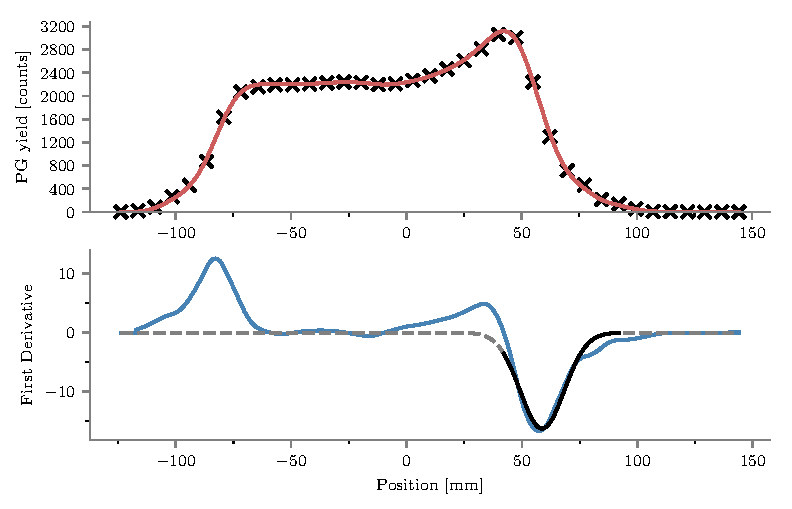
\includegraphics[width=.45\textwidth]{amv_mps_fow}}\quad
  \subfloat[KES]{\label{LinComparison}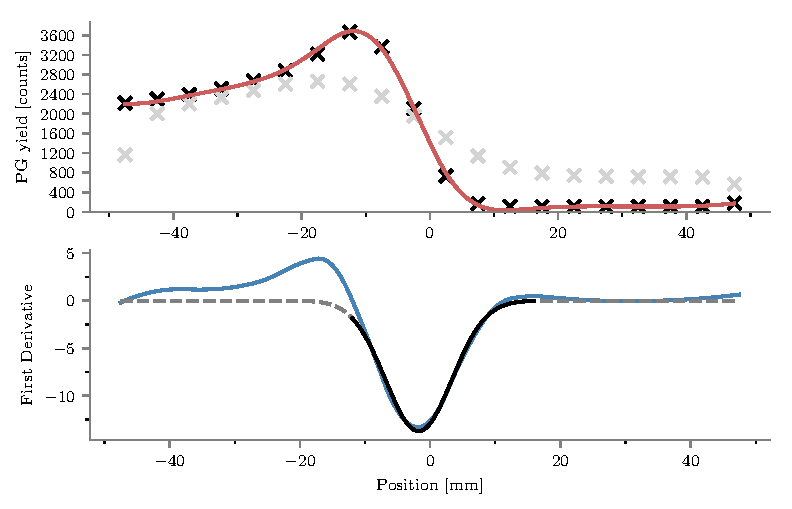
\includegraphics[width=.45\textwidth]{amv_kes_fow}}
  \caption{\label{PGprofileFairComp} MPS and KES comparisons with perfect absorber and the same energy (E>1 MeV) and no TOF selection. \ds{I wonder if the x scale could be the same for KES and MPS, it will allow better comparison and emphasis the difference in FOV}\bh{I remember doing this at some point (by plotting the curves in the same axis), but because they are quite different it became difficult to show each profile clearly. I prefer to keep it like it is, so that the profiles cover their axis maximally.}}
\end{figure}  

%Since the model does not explicitly deal with collimator transparency or absorber efficiency, we compare the AM to a Monte Carlo simulation with perfect absorber and collimator. Because such conditions are unphysical, results with a physical collimator and physical absorber are shown for the spatial resolution and detection efficiency respectively.

% The FOW shown in table~\ref{FOWCOMP} shows that both cameras perform similar with ToF selection. For the MPS the ToF selection makes no difference (up to 2\%), while for the KES it gives a 10-20\% improvement. The results are a bit worse than the calculated values in table~\ref{GeomFormulas}, but close to the 20 mm as postulated in \cite{Priegnitz2015}.

%When we make the collimator perfectly absorbing (any tracks entering the collimator material are killed), we observe the KES's effective slit width in action: the transmission through the collimator creating a wider $s_e$ is gone and we see the FOW decrease between 40 and 100\%. This is roughly in line with the calculated $s_e$. Surprisingly the FOW of the KES approaches the theoretical value nearly, while the MPS is still a few millimeters worse than calculated. 

%\answ{Table~\ref{tab:AMV} 1) We have in principle 4 combinations with real/perfect collimator and real/perfect absorber. I propose to use only two configuration for each measurement (Res and Eff). Res: real/perfect collimator with perfect absorber to see the influence of collimator transparency on Res. Eff: real/perfect absorber with perfect collimator to see the influence of the absorber intrinsic efficiency on the camera efficiency. 2) The discrepancy between the KES efficiencies obtained with AM and MC ($1.06 \cdot 10^{-3}$  vs $7.54\cdot10^{-4}$) has still to be understood.}


% \begin{table}
% \centering
% \begin{tabular}{lllllllll}
% 	\midrule
% 	Time selection 					& ToF &     &     &     & none&     &     &     \\
% 	Energy selection 				& 1   &     & 3   &     & 1   &     & 3   &     \\
% 	Camera 							& MPS & KES & MPS & KES & MPS & KES & MPS & KES \\
% 	\midrule
% % 	FOW                     	& 19.7& 20.9& 18.3& 19.3& 19.8& 21.9& 17.9& 23.6\\
%     FOW (both LYSO)            & 17.7 & 13.6 & 17.0 & 12.4 & 17.8 & 13.3 & 17.1 & 12.5 \\
% 
%  	FOW (perfect collimator) 	& 17.8& 13.7& 16.9& 13.7& 18.3& 14.2& 17.0& 11.6\\
% 	\midrule
% \end{tabular}
% \caption{FOW PSF.}
% \label{FOWCOMP}
% \end{table}

\begin{table}[h]
\centering
\begin{tabular}{lllllllll}
	\midrule
	\multicolumn{2}{c}{}				& \multicolumn{3}{c}{MPS}																	&& \multicolumn{3}{c}{KES}										\\
	\cline{3-5}\cline{7-9}
	\multicolumn{2}{c}{}				& AM 										& MC 									& RD	 			&& AM 										& MC							\\
	\midrule
	Res	& Perfect camera				& 14.5 mm								& \hl{22.5 mm} 	 			& \hl{35\%}	&& 13.5 mm								& 12.0 mm									& 13\%  \\
		& Phys. camera					& 					& 17.2 mm 	 					&						&& 23.7									& 19.3 mm									& 23\% \\

	\midrule
	Eff    & Perfect camera			&  $6.66 \cdot 10^{-4}$ & $6.49\cdot10^{-4}$	&	3\%					&& $1.06 \cdot 10^{-3}$  & $9.74\cdot10^{-4}$			& 9\%\\
	       & Phys. camera				&  $3.76 \cdot 10^{-4}$	& $6.61\cdot10^{-4}$	&	11\%					&& $6.03 \cdot 10^{-4}$	& \hl{$1.03\cdot10^{-3}$}	& \hl{73\%}\\
 	\midrule
	FRP    & Perfect camera			&  & 0.90 mm	&  &&  & 0.10 mm			& \\
	       & Phys. camera				&  & 0.26 mm	&  && 	& 0.33 mm	& \\
 	\midrule
\end{tabular}
\caption{MPS and KES detection efficiencies ("Eff") and spatial resolution ("Res") from analytical models and MC. The predictions of the analytical model (AM column) are derived from the equations of table~\ref{table:AMformulas}, at the center of the camera in the case of KES ($x=0$). MC data have been obtained with energy selection E>1~MeV. For the \enquote{Perfect camera} simulation, the collimator was adjusted to be 100\% opaque, and detection with perfect precision and 100\% efficiency. RD: relative deviation between AM and MC. \ds{Start rather by Perfect Cam instead of  Phys Cam}\bh{done}}
\label{tab:AMV}
\end{table}

Table~\ref{tab:AMV} compares the detection efficiency and the spatial resolution obtained from the analytical model and Monte Carlo simulations. \bh{What exactly is the emphasis in the table for? Should it be discussed here?}

\paragraph{Spatial Resolution} The results for the spatial resolution 

\paragraph{Efficiency}

\paragraph{Fall-off Retrieval position} The MC-obtained fall-off retrieval position is also given in table~\ref{tab:AMV}. The model does not predict FRP, but results are given to see the effect of switching from a perfect camera model to the physical one. The closeness of the results implies that for the MPS in particular the opacity of the collimator and quality of PG detection in the absorber don't have much room for improvement.

% \begin{figure}[htp]
%   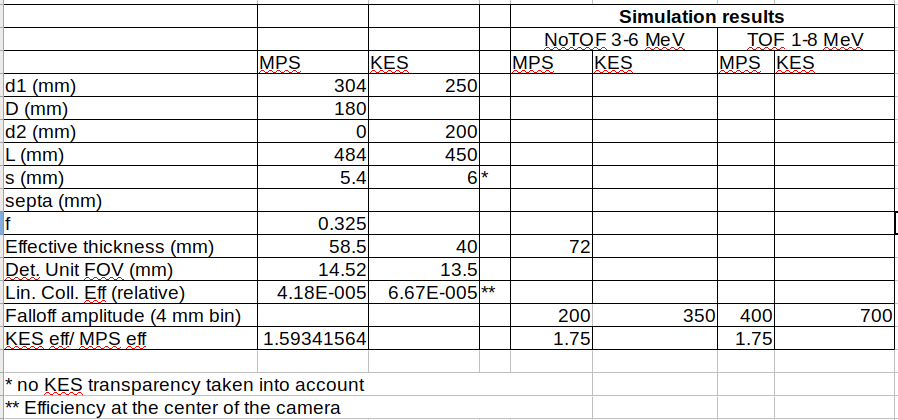
\includegraphics[width=\textwidth]{FairComparison}
%   \caption{\label{CameraPerformancesFairComp} MPS and KES comparisons with the same absorber, energy and TOF selection. The first columns of the table correspond to the geometrical calculations. \textcolor{red}{It is interesting to show the results for the two energy selections but it would be nice to have only one TOF selection (no TOF).}}
% \end{figure}

\subsection{Prototype Comparison}

Performance under clinical conditions is the primary purpose of these PG cameras, and therefore we include the results of the clinical case study. As described in table~\ref{table:CameraParameters}, we took settings and corresponding background estimates for the camera's published settings to simulate each camera as-is during measuremnts of the same PMMA phantom.

\subsubsection{PG profiles}

Figure~\ref{fig:PGprofileProtoComp} shows the PG profiles with $10^9$ protons, averaged over 50 runs. The averaging removes statistical fluctuations so that the base structure of the profiles can be best studied. The MPS camera is large enough to capture both the fall-off and fall-in positions, so the camera was displaced slightly (5cm in the distal direction) in order for the full profile to show up. The camera's are positioned on the PG production fall-off, so the expected fall-off is at +50mm and 0mm for the MPS and KES respectively.

\begin{figure}[!htp]
  \centering
  \subfloat[MPS]{\label{SmeetsComparison}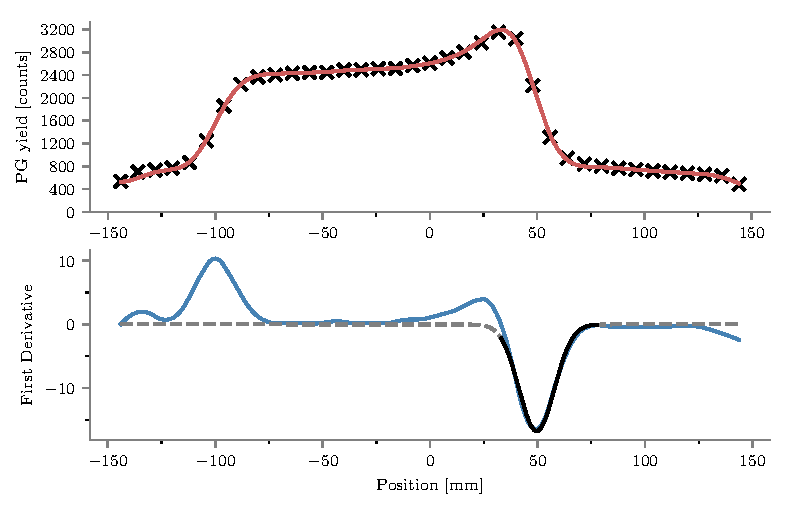
\includegraphics[width=.45\textwidth]{pc_mps_fow}}\quad
  \subfloat[KES]{\label{LinComparison}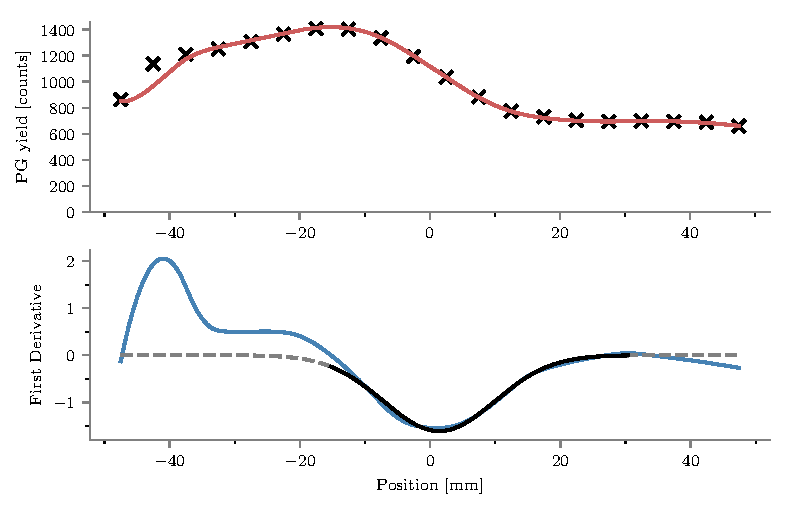
\includegraphics[width=.45\textwidth]{pc_kes_fow}}
  \caption{\label{fig:PGprofileProtoComp}MPS and KES prototypes comparisons. MPS BGO aborber with 1-8 MeV energy selection and TOF selection. KES: LYSO absorber with 3-6 MeV and no TOF selection. On the top row the reconstructed profiles, averaged over 50 simulation each with $10^9$ protons. On the bottom row in blue the first derivative of the profile, with in black the Gaussian fit in the fall-off region, with which the fall-off position and width will estimated. Note that the horizontal scales are different and correspond to each camera's field of view.}
\end{figure}  

We can see that, as expected, the MPS has higher PG counts, because of the wider energy selection (the PG production spectrum shows most production at lower energies). We see qualitatively the fall-off positions are at the expected coordinate, and that the BP is more pronounced in the MPS. At the tail end we see the backgrounds converge on roughly the same level. \bh{is this strange? I guess I've seen too many profile graphs to know this anymore ;)}

\begin{table}[h]
\centering
\begin{tabular}{llllll}
	\midrule
			& MPS					& KES \\
	\midrule
 	Res		& 19.4 mm				& 20.1 mm\\
	Eff  	& $1.04\cdot10^{-3}$	& $5.58\cdot10^{-4}$\\
 	\midrule
\end{tabular}
\caption{Detection efficiencies and spatial resolution of MPS and KES prototypes. Energy and TOF selection: E>1~MeV and TOF for MPS -- 3-6~MeV and no TOF for KES.}
\label{tab:ProtoPerformance}
\end{table}

Table~\ref{tab:ProtoPerformance} summarizes the spatial resolution and efficiency results. Even though the MPS had a more pronounced fall-off, we can see the spatial resolutions are roughly equivalent. \bh{Some comment on efficiency?}

\subsubsection{FRP}

\begin{figure}[!htp]
  \centering
  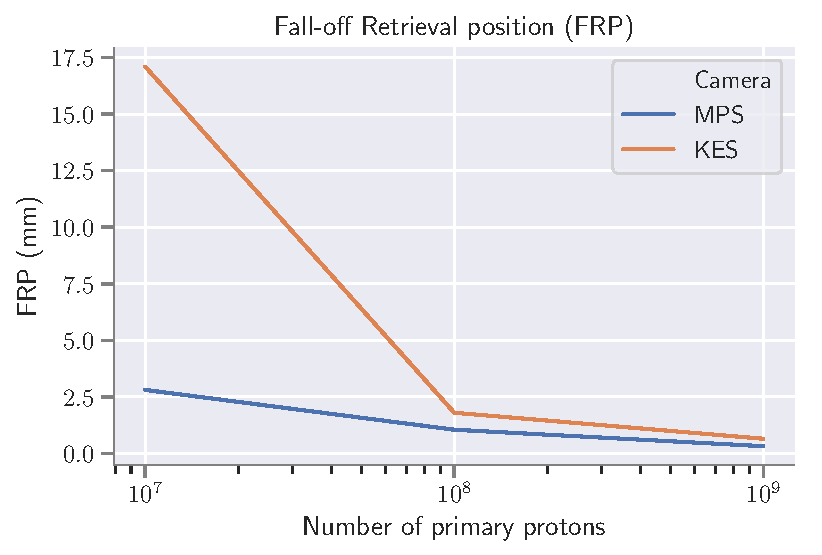
\includegraphics[width=.8\textwidth]{pc_frp_plot}
  \caption{\label{fig:PCFRPComp}Fall-off retrieval position comparison for the Prototype Comparison.}
\end{figure}

Figure showing the falloff retrieval precision (FRP) (standard deviation of the falloff position distributions) for the 2 prototypes as a function of the number of incident protons ($10^7$, $10^8$, $10^9$). As expected, more primaries translate to a better FRP. Both cameras achieve submillimetric accuracy at $10^9$ primaries, and millimetric precision with $10^8$ primaries. With fewer than $10^8 primaries$, the cameras, KES in particular, are outside the limits of interest of shift detection.

\begin{table}[h]
\centering
\begin{tabular}{llllllllll}
	\midrule
	Primaries & Time selection 					& ToF &     &     &     & none&     &     &     \\
	          & Energy selection 				& 1   &     & 3   &     & 1   &     & 3   &     \\
	          & Camera 							& MPS & KES & MPS & KES & MPS & KES & MPS & KES \\
	\midrule
 	$10^9$    & AMV perfect det.        & 0.90 & 0.10 & NTNE\\
% 	$10^9$    & AMV perfect det.        & ? & 0.44 & 0.49 & 0.52 & 0.42 & 0.40 & 0.45 & 0.55 \\
% 	$10^8$    & LYSO and no bg        & ? & 1.22 & 1.70 & 1.74 & 1.24 & 1.29 & 1.63 & 1.48 \\
% 	$10^7$    & LYSO and no bg        & ? & 4.03 & 5.88 & 5.65 & 3.76 & 4.89 & 5.65 & 10.76 \\
	\midrule
 	$10^9$    & detectors as proposed     & \textbf{0.32} & 0.56 & 0.36 & 0.57 & 0.31 & 0.60 & 0.46 & \textbf{0.65} \\
 	$10^8$    & detectors as proposed     & \textbf{1.05} & 1.69 & 1.30 & 1.96 & 1.04 & 1.93 & 1.34 & \textbf{1.80} \\
 	$10^7$    & detectors as proposed     & \textbf{2.81} & 7.96 & 3.65 & 12.9 & 2.96 & 14.8 & 19.3 & \textbf{17.1} \\
	\midrule
\end{tabular}
\caption{\bh{THIS TABLE IS TO BE REMOVED. REPLACED WITH FRP PLOT.}Fall-off retrieval precision (defined as the standard deviation of the FOP over the number of times the simulation is ran. In bold, the cuts and ToF selections as proposed.}
\label{FRPCOMP}
\end{table}

%%%%%%%%%%%%%%%%%%%%%%%%%%%%%%%%%%%%%%%%%%%%%%%%%%%%%%%%%%%%%%%%%%%%%%%%%%%%%%%%
\section{Discussion}

Mention the limitations of the KES: detection efficiency not constant over the FOV + limited FOV
\bh{Perhaps Etienne is most suited write this part.}


\subsection{Clinical implications}

It is often stated PG cameras will be able to be used to track deviations at the spot-level. The cameras in this study required $10^8$ primaries for an acceptable FRP. It is helpful to put this in clinical perspective, so we plot the structure of two treatment plans in figures \ref{fig:planmid} and \ref{fig:planhigh}. These treatmentplans were produced and used for two clinical cases, the former considered of medium complexity, which is to say a fairly typical plan, and the second of high complexity. It stands to reason that from a clincal point of view, treatment monitoring becomes more interesting as the complexity of the plan increases, because plans become more complex in more difficult or sensitive cases, where a correct planned and delivered dose are desirable.

\begin{figure}[htp]
  \centering
  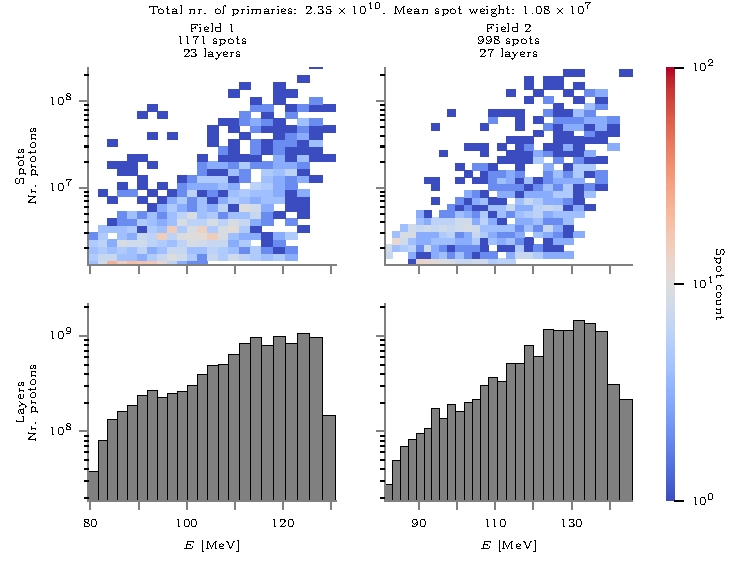
\includegraphics[width=0.8\linewidth]{MENINGIOMA_F1nonorm-plot}
  \caption{Treatmentplan for a Meningioma case, which is considered a plan-type of medium complexity. On top: the spots are binned as function of energy and spot weight (number of protons), with high spot counts in red (hot spots) and low spot counts in blue (cool spots).}
  \label{fig:planmid}
\end{figure}

\begin{figure}[htp]
  \centering
  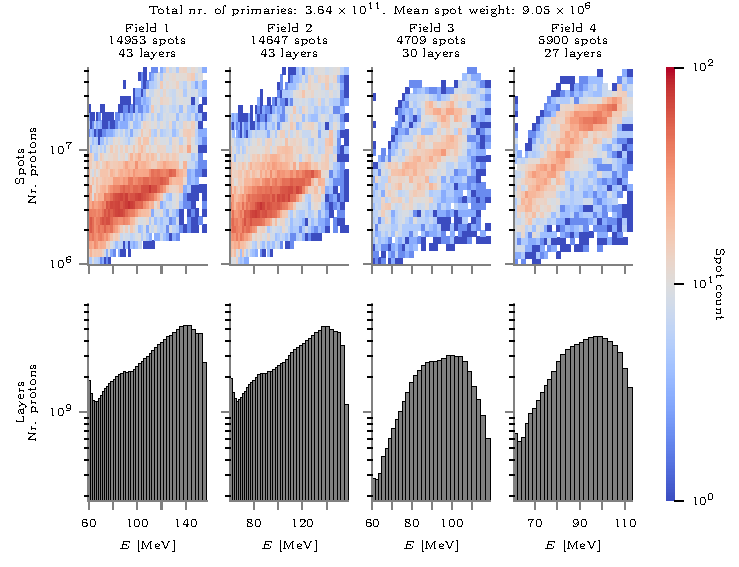
\includegraphics[width=0.8\linewidth]{CSI_F1nonorm-plot}
  \caption{Treatmentplan for a large and complex pediatric brain and spine case. The left two fields are for the brain, the right two for the spine. The color scale chosen the same as in figure \ref{fig:planmid}.}
  \label{fig:planhigh}
\end{figure}

From figures \ref{fig:planmid} and \ref{fig:planhigh} we can observe that spot-level monitoring is unlikely with the camera prototypes included in this study. In the complex case not a single spot has a prescription of $10^8$ protons or more. Fortunately, nearly all energy layers exceed $10^8$ primaries, so monitoring at the layer-level poses no issues for these cameras. Nevertheless, we hope the theoretical framework developed and validated in this paper will help move PG camera designs towards the realm where spot-level monitoring would become feasible.

%%%%%%%%%%%%%%%%%%%%%%%%%%%%%%%%%%%%%%%%%%%%%%%%%%%%%%%%%%%%%%%%%%%%%%%%%%%%%%%%
\section{Conclusion}

We have presented and validated an analytical model that relates the collimator dimensions of Prompt Gamma cameras to a predicted spatial resolution and detection efficiency. Two collimator designs are modelled: multi-parallel slit and knife edge. The validation consisted of Monte Carlo simulations of two current Prompt Gamma camaera prototypes, one of which has been employed in clinical setting. We also show the performance of these two prototypes in their proposed configuration with a mono-energetic spot in a PMMA phantom with background modelling. The prototypes reach millimetric precision with $10^8$ primaries or more. The fall-off retrieval position performance is put into clinical context.

%%%%%%%%%%%%%%%%%%%%%%%%%%%%%%%%%%%%%%%%%%%%%%%%%%%%%%%%%%%%%%%%%%%%%%%%%%%%%%%%
\section{Acknowledgements}

This work was partly supported by SIRIC LYric Grant INCa-DGOS-4664, LABEX PRIMES (ANR-11-LABX-0063 / ANR-11-IDEX-0007) and Fondation ARC. The authors would like to thank Marie-Claude Biston, Thomas Baudier and Gloria Vilches-Freixas for their help finding the CT images and making the treatment plan. We also thank Erik Almhagen and Uppsala University Hospital, Sweden for the treatment plan data presented in this paper.

%%%%%%%%%%%%%%%%%%%%%%%%%%%%%%%%%%%%%%%%%%%%%%%%%%%%%%%%%%%%%%%%%%%%%%%%%%%%%%%%
\newpage

\appendix
% \begin{appendices}
% 
%%%%%%%%%%%%%%%%%%%%%%%%%%%%%%%%%%%%%%%%%%%%%%%%%%%%%%%%%%%%%%%%%%%%%%%%%%%%%%%%

\section{Fall-off position and width estimation procedure}\label{sec:fopproc}

\subsection{Fall-off position estimation procedure}

From a clinical perspective, the range estimate could be more interesting than FOP, because it can distinguish simple offset errors from patient morphological change. While the MPS camera was conceived for whole range PG profile detection, the KES camera FoV was chosen for BP region PG detection only. To make the comparison fair, only the FOP could be considered. Multiple approaches to extracting a FOP from the line profile have been proposed \citep{Smeets2012,Gueth2013,Roellinghoff2014a,Janssen2014,Sterpin2015}. In preparatory work, a number of the proposed procedures were investigated. Significant sensitivity to free parameters on the final FOP estimates were seen. In summary, the FOP estimate depends greatly on the procedure, and often on having yields uncommon on the spot-level in clinical TPs, and also on an absence of unavoidable inhomogeneities.

Therefore the fitting method was not chosen as a topic for study in this paper. Instead, a simple method that works on most the data available to the authors was used: first a smoothed and interpolated spline function is fitted against the detected PG data points, after which a baseline and (distal) peak position are determined. The intersection of the spline with the half-height of the peak above the baseline is then taken as the FOP.


\begin{enumerate}[noitemsep]
\item The measured PG profile is smoothed and interpolated with a smoothing spline function:

\begin{equation}
\sum_{i=1}^n (y_i - \hat f(x_i))^2 + \lambda \int_{x_1}^{x_n} \hat f''(x)^2 \,dx
\end{equation}

where $y_i$ is the measured PG profile and $x_i$ the associated x-coordinates, $\hat f(x_i)$ the estimate smoothed spline function and $\lambda$ a smoothing parameter that determines the penalty for deviating from measurement in exchange for smoothness (second order derivatives are close to zero on smooth functions). $\lambda = 0$ produces a perfect spline fit to the data, while $\lambda \gg 1$ produces a horizontal line. We found that $\lambda = 2$ provided an acceptable trade-off between overfitting to noise and removing too many features, which tends to happen for low statistic measurements.
\item The obtained function is plotted for 1024 $x_j$, an number that provided a sufficiently high resolution. Any $f(x_j) < 0$ are set to $0$. 
\item The global maximum is found.
\item The baseline is set equal to the lowest 25\% of bins.
\item From the distal end backwards, the first maximum is taken as the distal most peak position, if it is above the threshold of 30\% of the difference between baseline and global maximum. If no such point is found, the global maximum is taken as the distal most maximum.
\item The fall-off amplitude (FOA) is set to the difference between the distal maximum and baseline: $FOA = max-baseline$. The FOP is obtained by traversing the smoothed profile from the distal end towards the peak until $y_j > \frac{1}{2}FOA$.
\end{enumerate}

The results of this procedure are illustrated in figure~\ref{fig:our-fit}. Every PG profile was estimated 50 times, and so we obtained 50 estimates for the FOP. It is assumed that the FOPs follow a Gaussian distribution, so the mean of the 50 realizations gives the best FOP estimate and the sigma gives the precision of the ability to estimate the best FOP. Comparing the 50 FOP estimates obtained from the CT with the 50 estimates obtained from the RPCT simulations, gives 2500 possible shift estimates. Again, the distribution of shifts should be centered at the true shift, while the sigma indicates how likely it is that this true shift is detected under the current conditions.

\begin{figure}[htp]
  \centering
  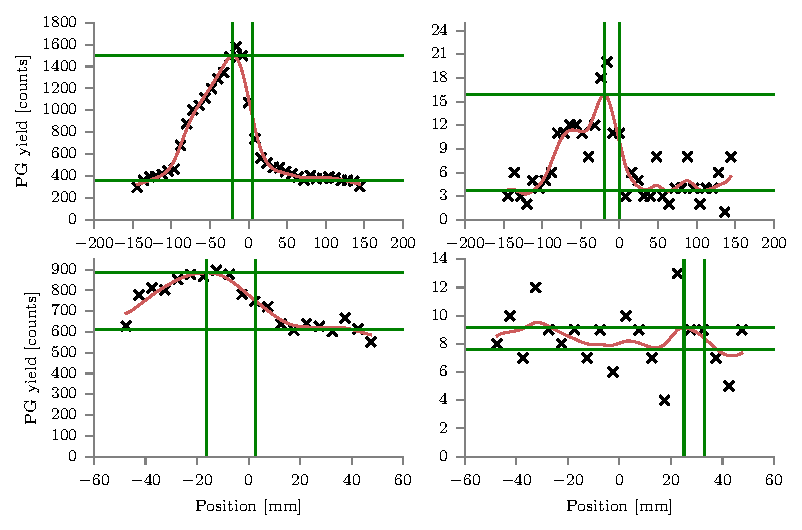
\includegraphics[width=0.9\linewidth]{fopproc}
  \caption{The top row demonstrates the fall-off determination procedure on the multi-parallel camera data; on the bottom row on knife-edge slit camera data. The left column is produced with a PG signal due to $10^9$ primaries, while the right column was produced with $10^7$ primary protons. In black crosses the measured PG counts are plotted. The smoothed data is shown in red. The green horizontal lines are drawn at the obtained distal maxima and baselines, while the vertical green lines shown the position of the distal maximum and the position of the fall-off. For the bottom-right plot, a history is visible where the procedure fails: the background induces an erroneous peak detection.}
  \label{fig:our-fit}
\end{figure}

\subsection{Fall-off width estimation procedure}

\begin{figure}[htp]
  \centering
  \subfloat[KES]{\label{FOWKES}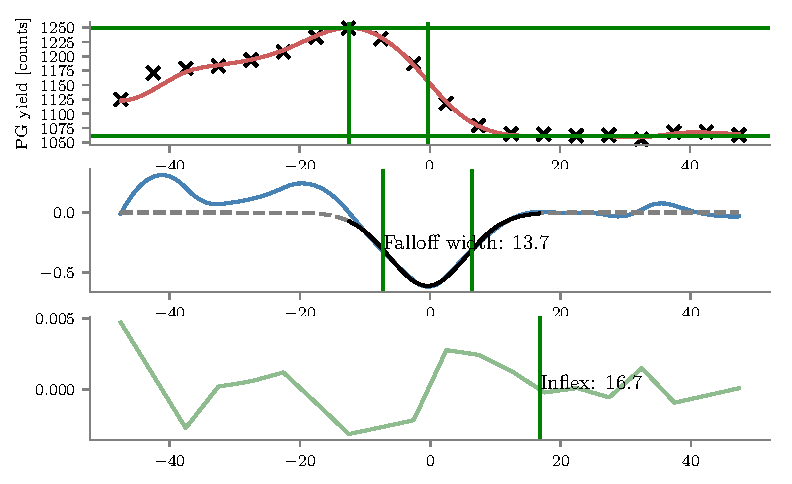
\includegraphics[width=.45\textwidth]{FOW_PMMA_phantom-iba-auger-tof-3}}\quad
  \subfloat[MPS]{\label{FOWMPS}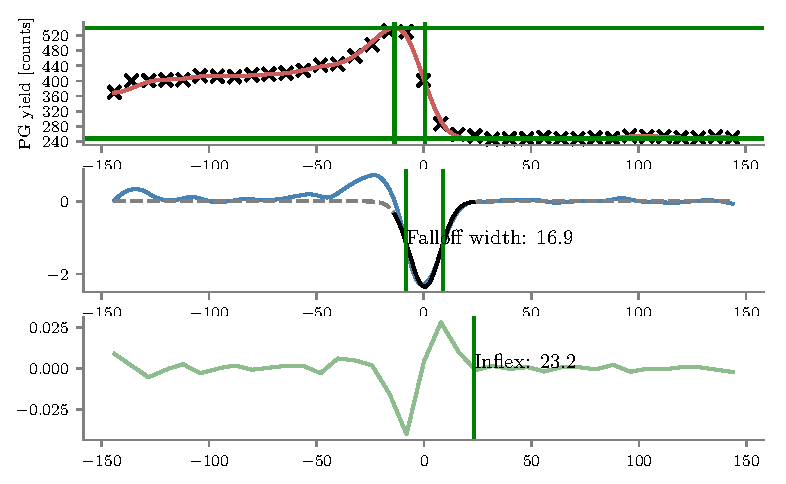
\includegraphics[width=.45\textwidth]{FOW_PMMA_phantom-ipnl-auger-tof-3}}
  \caption{\label{FOWILLUS} MPS and KES FOW estimation illustrated. \ds{idem x scale}}
\end{figure}

Figure~\ref{FOWILLUS} shows and illustration of the procedure for two selected profiles obtained with each collimator. To estimate the fall-off width (FOW), we smooth the profile in a similar manner as for the FOP estimation, as detailed in appendix~\ref{sec:fopproc} (row 1 in Figure~\ref{FOWILLUS}). Then, a first and second order derivative is computed. On the first order derivative, a Gaussian is fitted (dashed line on second row), on the interval (solid line) between the profile maximum (Bragg Peak) and the first inflection point past the FOP on the second order derivative (here the 1D PG profile is at the baseline of the background, see third row). The Gaussian is fit with a fixed offset of zero, because the baseline of the background is zero. The full width half max of the fitted Gaussian is then taken as the FOW (second row).

%%%%%%%%%%%%%%%%%%%%%%%%%%%%%%%%%%%%%%%%%%%%%%%%%%%%%%%%%%%%%%%%%%%%%%%%%%%%%%%%

\section{Verification of the cameras}

In \cite{Priegnitz2015} PG shifts due to beam energy shifts are studied for the KES camera: the \emph{detectability} of the fall-off as function of the number of primaries. Here that simulation was recreated: a mono-energetic beam shoots into a waterbox at two energies. 50 realizations are generated with a 139 MeV beam energy, and 50 realizations with 144 MeV. At $10^9$ primaries, the distributions are well separated with a shift of 8.3 mm (different from \cite{Priegnitz2015} because of the different material). In figure 13 in \cite{Perali2014} with $10^9$ primaries a standard deviation of 1.5 mm is obtained, while here 1.21 and 1.14 mm were obtained. It is sufficient agreement to be confident of our setup and further results.

The KES prototype's sensitivity to accurate positioning with respect to the expected FOP was elaborated upon in \citet[Section IV.A.3]{Sterpin2015}: the detector response is, due to the KES collimator, not linear as with a parallel slit collimator. In this study, to make the comparison as fair as possible and avoid any bias, alignment on the FOP specific for each spot was ensured as follows: the intermediate PG source image of vpgTLE (equivalent to the PG emission) was projected on the beam axis, and then convolved with a Gaussian of $\upsigma = 8.5$ mm, which corresponds to the point spread function (PSF) with a FWHM of 20 mm used in \cite{Priegnitz2015} to approximate the detected profiles from the emitted profile. These profiles will be referred to as "PG + PSF" profiles. As a matter of fact, the MPS prototype has roughly the same PSF as the KES prototype so that "PG + PSF" fall-off position can be considered as the expected position for both cameras.

To verify the implementation of the MPS camera, the precision on the FOP, obtained with the procedure outlined in the previous paragraph, is compared to earlier results. In the caption of figure 9 in \cite{Pinto2014a} it is stated that with $10^8$ primaries a standard deviation of 1.3 mm is obtained for the detector design used here, which is about 20\% different from the results obtained in this study: 1.63 and 1.54 mm.
%%%%%%%%%%%%%%%%%%%%%%%%%%%%%%%%%%%%%%%%%%%%%%%%%%%%%%%%%%%%%%%%%%%%%%%%%%%%%%%%
% \end{appendices}
\newpage

%%%%%%%%%%%%%%%%%%%%%%%%%%%%%%%%%%%%%%%%%%%%%%%%%%%%%%%%%%%%%%%%%%%%%%%%%%%%%%%%

\bibliographystyle{plainnat}
\bibliography{lib.bib}
\end{document}%\grid
